%Template preso da il professore tommaso rigon

\documentclass[12pt, a4paper, twoside, openright]{book} 
\usepackage[top=2.5cm, bottom=2.5cm, left=3cm, right=3cm]{geometry}

\usepackage[english]{babel} 
\usepackage[T1]{fontenc}
\usepackage[utf8x]{inputenc} % Serve per le lettere accentate
\usepackage{mathtools} % per valore assoluto e norma
\usepackage{graphicx} % Comandi aggiuntivi per la gestione delle immagini
\usepackage{url} % per scrivere gli indirizzi Internet
\usepackage{booktabs,subcaption} % Tabelle
\usepackage{amsthm,amsmath,amssymb,mathrsfs,dsfont}
\usepackage{rotating}
\usepackage[font=itshape,noorphans]{quoting}
\usepackage{bm,bbm}
\usepackage{microtype}
\usepackage{float}
\microtypesetup{protrusion=true,expansion=true}

\usepackage{hyperref}
\usepackage[dvipsnames]{xcolor}

\usepackage{tikz}
\usetikzlibrary{fit,calc,positioning,shapes,shadows,arrows}
\tikzset{font={\fontsize{10pt}{12}\selectfont},
hidden/.style = {
		draw = black ,
        shape = circle,
        inner sep = 11pt
    },
controlled/.style = {
		draw = black ,
        shape = rectangle,
        inner sep = 11pt
    } }

\usepackage{scrextend}
\usepackage[ruled,norelsize,vlined]{algorithm2e}

\usepackage[round]{natbib}
\usepackage[nottoc]{tocbibind}
\addto\captionsenglish{\renewcommand{\bibname}{Bibliografia}}


\usepackage[small]{titlesec}

\usepackage{caption}
\captionsetup{labelfont={bf},font=small}
\captionsetup[sub]{font=small,labelfont={bf}}

\usepackage{setspace}
\onehalfspacing
\linespread{1.3}

%These commands assume a very low tolerance for spacing between paragraphs
\usepackage[all]{nowidow} % Somewhat extreme, but it avoids widow rows
\pretolerance=0
\lineskip=0pt \lineskiplimit=0pt %
\tolerance=2000 \hyphenpenalty=300 \exhyphenpenalty=300%
\doublehyphendemerits=100000%
\finalhyphendemerits=\doublehyphendemerits
 

\usepackage[osf]{mathpazo} % add possibly `sc` and `osf` options
\usepackage[euler-digits]{eulervm}
\usepackage[scaled=0.85]{beramono}
\DeclareSymbolFont{greekletters}{OML}{cmr}{m}{it}
\DeclareMathSymbol{\varrho}{\mathalpha}{greekletters}{"25}
\DeclareMathSymbol{\varsigma}{\mathalpha}{greekletters}{"26}

% COlors
\definecolor{webgreen}{rgb}{0,0.5,0}
\definecolor{webbrown}{rgb}{0.6,0,0}
\definecolor{structural}{RGB}{0,0, 130}   % Structural


%%%%%%%%%%%%%%%%%%%%%%%%%%%%%
%Opzioni pacchetto Fancyhdr
%%%%%%%%%%%%%%%%%%%%%%%%%%%%%

\usepackage{fancyhdr}

\pagestyle{fancy}
\setlength{\headheight}{15pt}
% i comandi seguenti impediscono la scrittura in maiuscolo
% dei nomi dei capitoli e dei paragrafi nelle intestazioni
\renewcommand{\chaptermark}[1]{\markboth{#1}{}}
\renewcommand{\sectionmark}[1]{\markright{\thesection\ #1}}
\fancyhf{} % rimuove l'attuale contenuto dell'intestazione
\fancyhead[LE,RO]{\thepage \sffamily}
\fancyhead[LO]{Capitolo \thechapter. \textit{\leftmark}}
\fancyhead[RE]{Capitolo \thechapter. \textit{\leftmark}}
\renewcommand{\headrulewidth}{0.5pt}
\renewcommand{\footrulewidth}{0pt}

% Acknloedgments settings
\newenvironment{acknowledgements}% 
{\cleardoublepage\null\vfill\begin{center} %
\bfseries Ringraziamenti\end{center}} %
{\vfill\null}

%*********************************************************************************
% Nuovi ambienti: definizioni, teoremi etc. etc.
%*********************************************************************************
\usepackage{amsthm}
% definizioni (serve il pacchetto amsthm)
\newtheoremstyle{classicdef}% Nome
{12pt}% Spazio che precede l’enunciato
{12pt}% Spazio che segue l’enunciato
{}% Stile del font dell’enunciato
{}% Rientro (se vuoto, non c’è rientro,
% \parindent = rientro dei capoversi)
{\scshape}% Stile del font dell’intestazione
{:}% Punteggiatura che segue l’intestazione
{.5em}% Spazio che segue l’intestazione:
% " " = normale spazio inter-parola;
% \newline = a capo
{}% Specifica l’intestazione dell’enunciato
% (normalmente viene lasciata vuota)

\theoremstyle{definition}
\newtheorem{assumption}{Assumption}
\numberwithin{assumption}{chapter}

\theoremstyle{definition}
\newtheorem{definition}{Definition}
\numberwithin{definition}{chapter}

\theoremstyle{remark}
\newtheorem{example}{Example}
\numberwithin{example}{chapter}

\theoremstyle{remark}
\newtheorem{remark}{Remark}
\numberwithin{remark}{chapter}


% teoremi (serve il pacchetto amsthm)
\newtheoremstyle{classicthm}% Nome
{12pt}% Spazio che precede l’enunciato
{12pt}% Spazio che segue l’enunciato
{\itshape}% Stile del font dell’enunciato
{}% Rientro (se vuoto, non c’è rientro,
% \parindent = rientro dei capoversi)
{\scshape}% Stile del font dell’intestazione
{:}% Punteggiatura che segue l’intestazione
{.5em}% Spazio che segue l’intestazione:
% " " = normale spazio inter-parola;
% \newline = a capo
{}% Specifica l’intestazione dell’enunciato
% (normalmente viene lasciata vuota)

\theoremstyle{plain}
\newtheorem{theorem}{Teorema}
\numberwithin{theorem}{chapter}

\newtheorem{corollary}{Corollario}
\numberwithin{corollary}{chapter}

\newtheorem{lemma}{Lemma}
\numberwithin{lemma}{chapter}

\newtheorem{proposition}{Proposizione}
\numberwithin{proposition}{chapter}

\newtheorem{ass}{Assumption}
\numberwithin{ass}{chapter}

%*********************************************************************************
% Impostazioni di hyperref
%*********************************************************************************
\hypersetup{%
    % hyperfootnotes=false,pdfpagelabels,
    %draft,	% = elimina tutti i link (utile per stampe in bianco e nero)
    colorlinks=true, linktocpage=true, pdfstartpage=1, 
    % decommenta la riga seguente per avere link in nero (per esempio per la stampa in bianco e nero)
    % colorlinks=false, linktocpage=false, pdfborder={0 0 0}, pdfstartpage=1, pdfstartview=FitV,%
    breaklinks=true, pdfpagemode=UseNone, pageanchor=true, pdfpagemode=UseOutlines,%
    plainpages=false, bookmarksnumbered, bookmarksopen=true, bookmarksopenlevel=1,%
    hypertexnames=true, pdfhighlight=/O,%nesting=true,%frenchlinks,%
    urlcolor=webbrown, linkcolor=Maroon, citecolor=structural, %pagecolor=RoyalBlue,%
    %urlcolor=Black, linkcolor=Black, citecolor=Black, %pagecolor=Black,%
}

%%%%%%%%%%%%%%%%%%%%%%%%%%%%%%%%%%%
% Definizione di alcuni parametri
%%%%%%%%%%%%%%%%%%%%%%%%%%%%%%%%%%%

\graphicspath{{img/}} % Directory delle immagini

%%%%%%%%%%%%%%%%%%%%%%%%%%%%%%%%%%
% INIZIO DEL DOCUMENTO
%%%%%%%%%%%%%%%%%%%%%%%%%%%%%%%%%%

\begin{document}

\frontmatter

\pagestyle{empty}



\pagestyle{empty} 

\begin{titlepage}
  
 \begin{center}
 {\large  

 \hfill

 \vfill
 {
 {\Large \textsc{Università degli studi di Milano--Bicocca}}\\
 {\textsc{Scuola di Economia e Statistica}}\\
 \vfill
	\textsc{Corso di Laurea  in} \\
	\textsc{Scienze Statistiche ed Economiche} \\
	\vfill
	\includegraphics[width=4cm]{front}
 \vfill
 
 {\Huge\color{Maroon}\textsc{Bayesian Causality}}\\
 }
}
\end{center}

\vfill
{
\large
\begin{flushleft}
\textsc{Relatore}: Dott. Stefano Peluso \\
\end{flushleft}

\vfill
\begin{flushright}
\textsc{Tesi di laurea di}:\\
 Simone Maria Gervasoni\\
\textsc{Matricola N. 880068}
\end{flushright}

\vfill
\begin{center}
\textsc{Anno Accademico 2024/2025S}
\end{center}

%\vfill
%\begin{flushright}
%\textsc{\today}
%\end{flushright}
}
\end{titlepage}


% Lista dei contenuti

\tableofcontents


\begin{acknowledgements}
Inserire qui gli eventuali ringraziamenti, altrimenti eliminare 
\end{acknowledgements}

\cleardoublepage

\mainmatter

\pagestyle{fancy}

\chapter{Introduzione}
\label{chapt:History Causality}
The problem of causality is of fundamental interest and it has been for as long as humans have been around. We always have asked why something happens and we tried many possible answers. The question of causality has been explored by philosopher and scientist alike, but its precise statistical definition has remained elusive until the seventies, when Rubin expanded and perfected a theory proposed by Neyman in 1932. This model diverges in a few key points from the definition of some philosopher; John Stuart Mill defines causality as  “the antecedent, or the concurrence of antecedents, on which [a given phenomenon] is invariably and unconditionally consequent”. Mill thinks that A causes B if and only if each time A happens than B happens. This kind of intuition not only is wrong but can be outright dangerous. Instead in this thesis we rely on the potential outcome model that we believe gives more satisfactory answers to the aleatory nature of reality.

\chapter{DAGs}
\label{chapt:DAGs}

Introduciamo come primo argomento i DAGs o Directed Acyclic Graph, questi servono per schematizzare relazioni di causalità, che non verrà  
definità rigorosamente ora ma affrontata nel capitolo \ref{chapt:PotentialOM}.
Un DAG è un grafo formato da vertici che rappresentano le variabili in analisi e da archi che rappresentano la relazione di causalità le variabili. Viene detto aciclico perché partendo da un vertice e seguendo gli archi non si può tornare su  quel vertice. Questi grafi non sono in grado di descrivere causalità reciproca simultanea $A \leftrightarrow B $  o feedback loop $A \rightarrow B \rightarrow A$ a meno che si inserisca un ulteriore vertice con lo stesso nome, anche se in questi casi non si consiglia di utilizzare questo tipo di grafici
\citep{cunningham2021causal}.

\begin{figure}[ht]
  \subcaptionbox{Non valid DAG}[.22\linewidth]{%
	\begin{tikzpicture}
		\node (A) at (0,0) {$A$};
    		\node (B) at (1,0) {$B$};
    		\path[<-] (A) edge (B);
    		\path[->] (B) edge (A);
	\end{tikzpicture}
  }%
  \subcaptionbox{Non valid DAG}[.22\linewidth]{%
	\begin{tikzpicture}
		\node (A) at (0,0) {$A$};
    		\node (B) at (1,0) {$B$};
    		\path[<-] (A) edge (A);
    		\path[->] (B) edge (A);
	\end{tikzpicture}
  }
  \subcaptionbox{Valid DAG}[.22\linewidth]{%
	\begin{tikzpicture}
		\node (A) at (0,0) {$A$};
    		\node (B) at (1,0) {$B$};
    		\node (C) at (2,0) {$C$};
    		\path[<-] (A) edge (B);
    		\path[->] (B) edge (C);
    		
	\end{tikzpicture}
  }%
	\label{validDAG}

\end{figure}
(I grafi sono da rifare)

Bisogna inoltre dire che i DAGs, essendo dei grafi sono di natura più sintetici, contengono molte informazioni non solo grazie agli archi disegnati ma anche grazie a quelli \textbf{non} disegnati, ad esempio il DAG \ref{validDAG} implica che $A \perp\!\!\!\perp C$ visto che non esiste un arco che li colleghi. 

 %Bisogna essere molto vigili delle assunzione nascoste di un DAG.



\section{Vertici e Archi}
Fare breve cappello

\subsection{Vertici}

Poniamo la C come la variabile \textit{outcome} cioè la variabile di interesse per l'indagine (la salute dopo un determinato intervento). Poniamo A come la variabile \textit{exposure} cioè quella di cui vogliamo quantificare l'effetto causale sulla variabile \textit{outcome} (per esempio che tipo di intervento viene proposto). Analizziamo quindi un singolo vertice in questo caso B, gli unici modi in cui si può collegare ad A e C sono i seguenti: 
\begin{figure}[H]
\centering    
	\begin{tikzpicture}
		\node (A) at (0,0) {$A$};
    		\node (B) at (1,1) {$B$};
    		\node (C) at (2,0) {$C$};
		\path[->] (A) edge (B);
    		\path[<-] (B) edge (C);
    		\path[->] (A) edge (C);
	\end{tikzpicture}
\caption{DAG: Common effect}
\label{DAG:Common effect}
\end{figure} 
\begin{figure}[H]
	\centering
	\begin{tikzpicture}
		\node (A) at (0,0) {$A$};
    		\node (B) at (1,1) {$B$};
    		\node (C) at (2,0) {$C$};
    		\path[->] (A) edge (B);
    		\path[->] (B) edge (C);
		\path[->] (A) edge (C);
	\end{tikzpicture}
\caption{DAG: Mediator}
\label{DAG:Mediator}
\end{figure} 
\begin{figure}[H]
	\centering
	\begin{tikzpicture}
		\node (A) at (0,0) {$A$};
    		\node (B) at (1,1) {$B$};
    		\node (C) at (2,0) {$C$};
    		\path[<-] (A) edge (B);
    		\path[->] (B) edge (C);
    		\path[->] (A) edge (C);
	\end{tikzpicture}
\caption{DAG: Common cause}
\label{DAG:Common cause}
\end{figure}
Dunque B nel grafico \ref{DAG:Common effect} viene chiamato \textit{collider}, mentre nei grafici \ref{DAG:Mediator} e \ref{DAG:Common cause} viene definito \textit{non collider}, mentre solo \ref{DAG:Common cause} come \textit{confounder}.
Infatti se volessimo quantificare la relazione causale tra A e C quando B è un \textit{non collider} o  un \textit{confounder} risulta più difficoltoso perchè sappiamo che B introduce  sistematicamente correlazioni spurie tra A e C (bisogna capire meglio come affrontare i mediators [bisogna controllarli?], osservazione più giusta per i ). Invece nel caso mostrato in figura \ref{DAG:Common effect} potremmo interpretare il $\hat{\delta}$ della regressione lineare:
\begin{equation}
C_i= A_i\delta + \epsilon_i
\end{equation}
come quantificazione dell'effetto causale che A ha su C, questo lo possiamo affermare solo dopo aver confermato che effettivamente:
\begin{itemize}
\item il grafo soddisfa \textit{Backdoor criterion} ( paragrafo \ref{sect:backdoor})
\item La direzione della causalità è corretta
\end{itemize}

\subsection{Archi}
definizione di path
definizione di open backdoor 
elenco di tutte le path possibili  con esempio




% magari metterli di fianco
%\begin{figure}[ht]
%  \subcaptionbox{First subfigure}[.22\linewidth]{%
%	\begin{tikzpicture}
%		\node (A) at (0,0) {$A$};
%    		\node (B) at (1,0) {$B$};
%    		\node (C) at (2,0) {$C$};
%    		\path[<-] (A) edge (B);
%    		\path[->] (B) edge (C);
%	\end{tikzpicture}
%  }%
%  \hfill
%  \subcaptionbox{Second subfigure}[.22\linewidth]{%
%	\begin{tikzpicture}
%		\node (A) at (0,0) {$A$};
%    		\node (B) at (1,0) {$B$};
%    		\node (C) at (2,0) {$C$};
%    		\path[<-] (A) edge (B);
%    		\path[->] (B) edge (C);
%	\end{tikzpicture}
%  }
%  \subcaptionbox{First subfigure}[.22\linewidth]{%
%	\begin{tikzpicture}
%		\node (A) at (0,0) {$A$};
%    		\node (B) at (1,0) {$B$};
%    		\node (C) at (2,0) {$C$};
%    		\path[<-] (A) edge (B);
%    		\path[->] (B) edge (C);
%	\end{tikzpicture}
%  }%
%
%\end{figure}

\section{Back door criterion}
\label{sect:backdoor}


\section{Collider Bias}
\begin{figure}[H]
\centering
	\begin{tikzpicture}
		\node (A) at (0,0) {$A$};
    		\node (B) at (1,1) {$B$};
    		\node (C) at (2,0) {$C$};
		\path[->] (A) edge (B);
    		\path[<-] (B) edge (C);
    		\path[->] (A) edge (C);
	\end{tikzpicture}
\caption{DAG:collider bias}
\label{DAG:Colliderbias}
\end{figure} 

 
\chapter{Potential outcome model}
\label{chapt:PotentialOM}

Il potential outcome model definisce l'effetto causale di un evento A come la differenza tra i due "stati" del mondo, cioè il mondo dove accade A e il mondo dove non accade A.

Poniamo ad esempio di voler capire se veramente un medicinale possa migliorare il mal di testa. Formalizziamo il problema ponendo X come l'insieme di covariate dei pazienti, D il regime di trattamento (che assume il valore 1 se viene dato il medicinale mentre assume valore 0 quando al paziente viene somministrato il placebo) e $Y^{obs}_i$ come il numero di minuti per cui persiste il mal di testa. 
Dunque se potessimo conoscere contemporaneamente  $Y^{obs}_i|D=1$ , che chiameremo $Y^{1}_i$, e $Y^{obs}_i|D=0$ , che chiameremo $Y^{0}_i$, allora calcolare se il medicinale causa un miglioramento risulterà molto semplice. Introduciamo un esempio numerico : 
\begin{table}[H]
\centering
\begin{tabular}{|c|c|c|c|c|}
\hline
Age & Sex & $Y^{0}_i$ & $Y^{1}_i$ & $\delta_i$ \\ \hline
20 & M & 20 & 21 & -1  \\ \hline
20 & F & 15 & 3 & 12 \\ \hline
20 & M & 8 & 10 & -2 \\ \hline
20 & F & 16 & 15 & 1 \\ \hline
30 & M & 12 & 13 & -1 \\ \hline
30 & F & 8 & 5 & 3 \\ \hline
30 & M & 2 & 11 & -9  \\ \hline
30 & F & 15 & 26 & 11 \\ \hline
\end{tabular}
\caption{Tabella esperimento }
\end{table}
Vediamo che il $\delta$ non è sempre positivo dunque la medicina non ha migliorato la situazione per tutti, notiamo però che in generale ha ridotto il tempo del malessere, questo però non basta, dobbiamo essere più precisi quantificando esattamente la tipologia e la dimensione dell'effetto.

\paragraph{Definizione parametri} \hspace{0pt} \\
\label{parag:param}
Definiamo quindi alcune quantità che ci risulteranno utili : 
\begin{itemize}
\item CATE o Conditional Average Treatment Effect è definito come $E[Y^{1}_i- Y^{0}_i|X] = E[\delta_i|X]$, quindi $CATE_{(M,20)}=E[\delta_i|X=(M,20)] \approx \frac{18-2}{2}=8$ , possiamo quindi dire che tra i maschi ventenni la medicina causa in media una riduzione di 8 minuti nella durata del mal di testa .
\item ATE o Average Treatment Effect è definito come  $E[Y^{1}_i- Y^{0}_i] = E[\delta_i]$, quindi $ATE= E[\delta_i] \approx \frac{18+12-2+18+3-9+11}{8}$.
\item ATT o Average Treatment on the Treated è definito come  $E[Y^{1}_i- Y^{0}_i|D=1] = E[\delta_i|D=1]$ 
\item ATU o Average Treatment on the Untreated è definito come 
$E[Y^{1}_i- Y^{0}_i|D=1] = E[\delta_i|D=1]$
\end{itemize}
 
Non possiamo calcolare gli ultimi due perché siamo ancora nel caso ipotetico dove conosciamo i due potential outcomes.
Ovviamente questa tabella non potrà mai essere riempita come abbiamo mostrato sopra perché possiamo veramente conoscere una sola quantità tra $Y^0_{i}$ e $Y^1_{i}$, sarà quindi impossibile avere certezza sulle quantità definite prima ma bisognerà stimarle. 
Dunque è utile fare la distinzione tra i valori \textit{fattuali} cioè cosa è veramente successo e \textit{controfattuale} cioè cosa sarebbe accaduto se il regime di trattamento fosse stato diverso.
Possiamo capire meglio la relazione tra potential outcome e observed outcome attraverso la  "switching equation": 
\begin{equation}
Y_i^{obs} = D_i \cdot Y^1_i + (1-D_i) \cdot Y^0_i
\label{eq:switching}
\end{equation}
Vediamo quindi che $Y_i^{obs} = Y^1_i$ quando $D_i =1$ ,mentre $Y_i^{obs} = Y^0_i$ quando $D_i = 0$. 
Bisogna precisare che la differenza tra $Y_i^{obs}$ e $Y^0_i,Y^1_i$ è che i primi sono valori effettivi, empirici che si possono osservare mentre gli ultimi sono valori ex-ante e dunque esistono prima che la $D_i$ venga somministrata.

Quello che invece ci ritroveremo nella realtà sarà una tabella più simile a questa 
\begin{table}[H]
\centering
\begin{tabular}{|c|c|c|c|}
\hline
Age & Sex & $Y^{0}_i$ & $Y^{1}_i$ \\ \hline
20 & M & 20 & ?  \\ \hline
20 & F & 15 & ? \\ \hline
20 & M & ? & 10 \\ \hline
20 & F & ? & 15  \\ \hline
30 & M & 12 & ? \\ \hline
30 & F & 8 & ? \\ \hline
30 & M & ? & 11   \\ \hline
30 & F & ? & 26 \\ \hline
\end{tabular}
\caption{Tabella esperimento }
\end{table}
Abbiamo dunque ridotto il problema della causalità ad un problema di \textit{Missing Data}, questa è la forza del modello usato.

\section{Studi randomizzati: Ruolo della randomizzazione}
Spesso si sente parlare di studi clinici randomizzati controllati, cioè studi in cui a metà dei partecipanti viene dato un placebo e all'altra metà il medicinale che è oggetto di studio, ovviamente né i medici né i pazienti sono a conoscenza di quali persone hanno assunto una o l'altra cosa. La situazione può essere espressa con un DAG in questa maniera: 
\begin{figure}[H]
\centering
	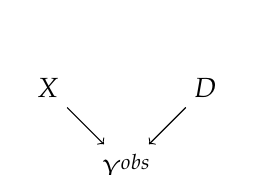
\begin{tikzpicture}
		\node (x) at (0,1) {$X$};
    		%\node (yz) at (0,0) {$Y^{1}$};
    		%\node (yo) at (2,0) {$Y^{0}$};
		\node (y) at (1,0) {$Y^{obs}$};
    		\node (D) at (2,1) {$D$};
    		%\path[->] (x) edge (yz);
    		%\path[->] (x) edge (yo);
    		\path[->] (x) edge (y);
    		%\path[<-] (T) edge (x);
    		\path[->] (D) edge (y);
	\end{tikzpicture}
\caption{Dag per studio randomizzato}
\label{fig:dag_random_EX}
\end{figure}
Ma perché questo procedimento è ormai la norma per verificare l'efficacia di un farmaco? E cosa ci può dire veramente un esperimento del genere? Sotto il potential outcome model questo procedimento può essere formalizzato tramite questa indipendenza
\begin{equation}
D \perp\!\!\!\perp (Y^{0},Y^{1})
\end{equation}
\label{eq:indipendence_r}

ciò significa che il trattamento non è amministrato in base ai potential outcome, ma in modo casuale. Non bisogna però confondersi e pensare che ciò implichi che $D \perp\!\!\!\perp Y^{obs}$, infatti ciò è espressamente falso ogni volta che il medicinale ha effetto su $Y^{obs}$.
Grazie all'equazione \ref{eq:indipendence_r} abbiamo che $E[Y^1_i] = E[Y^{1}_i | D_i = 1]  $ e la stessa cosa per $E[Y^0_i] = E[Y^{0}_i | D_i = 0] $.
Possiamo quindi dire che :
\begin{align}
ATE &= E[Y^1_i-Y^0_i ] \\ 
 &= E[Y^{1}_i | D_i = 1]- E[Y^{0}_i | D_i = 0]\label{eq:ATE_R} \\
	& =E[Y^{1}_i | D_i = 1]- E[Y^{0}_i | D_i = 1] \label{eq:ATT_R} \\
 &= E[Y^{1}_i | D_i = 0]- E[Y^{0}_i | D_i = 0] \label{eq:ATU_R}
  \end{align}

Nell'equazione \ref{eq:ATE_R} entrambi gli addenti sono quantità \textit{fattuali}, grazie alla legge dei grandi numeri stimiamo queste quantità con delle semplici medie, chiameremo quindi SDO la semplice differenza delle media osservate per i gruppi:
$$SDO = \frac{1}{N_1}\sum_{i:d_i=1}y_i - \frac{1}{N_2}\sum_{i:d_i=0}y_i \overset{\underset{\mathrm{(N_1, N_2) \rightarrow \infty}}{}}{=} ATE$$

Dall'equazione \ref{eq:ATT_R} e \ref{eq:ATU_R} possiamo concludere che nel caso randomizzato avremo che $ATE = ATT = ATU$.


\section{Studi osservazionali (?)} % esiste il termine?
Gli studi osservazionali (?) sono invece strutturati in modo diverso, i ricercatori osservano e raccolgono dati su individui o gruppi senza intervenire o manipolare alcun aspetto dell'ambiente di studio, per 2 motivi principali:
\begin{enumerate}
\item Potrebbe essere non etico o pratico dividere la popolazione in maniera casuale (immaginiamo di volere studiare se fumare causa un aumento nel rischio del cancro)
\item Gli eventi sono già accaduti (immaginiamo di volere studiare se i tassi di interesse incidano sul consumo)
\end{enumerate}

Dunque la cosa principale che cambia dal caso precedente è che $D \not \perp\!\!\!\perp (Y^{0},Y^{1})$, possiamo dunque rappresentare la situazione con il seguente DAG:
\begin{figure}[!h]
\centering
	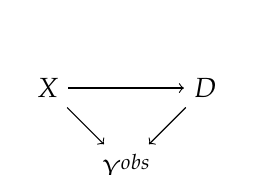
\begin{tikzpicture}
		\node (x) at (0,1) {$X$};
    		%\node (yz) at (0,0) {$Y^{1}$};
    		%\node (yo) at (2,0) {$Y^{0}$};
    		\node (y) at (1,0) {$Y^{obs}$};
    		\node (D) at (2,1) {$D$};
    		%\path[->] (x) edge (yz);
    		%\path[->] (x) edge (yo);
    		\path[->] (x) edge (D);
    		\path[->] (x) edge (y);
    		\path[->] (D) edge (y);
    		%\path[<-] (T) edge (x);
    		%\path[->] (T) edge (y);
	\end{tikzpicture}
\caption{Dag per studio osservazionale}
\label{fig:dag_OBS}
\end{figure}
%\citet{pacesalvan}

%\backmatter

\cleardoublepage
%\addcontentsline{toc}{chapter}{References}

\fancyhf{} % rimuove l'attuale contenuto dell'intestazione
\fancyhead[LE,RO]{\thepage \sffamily}
\fancyhead[LO,RE]{\textit{Bibliografia}}

\bibliographystyle{biblio_style.bst}
\bibliography{biblio} %Bibliography file
\nocite{*} 

\end{document}


